% IEEE Conference Template v1.1 (2026/11/02)
% Requires ieeeconf.cls v1.1.

% Document class:
%   Default: \documentclass{ieeeconf}  % 10pt, cameraready
%
% Modes:
%   singleanonymous  review mode (authors visible, line numbers)
%   doubleanonymous  review mode (authors hidden, line numbers)
%   cameraready      camera-ready mode (authors visible) (default)
%
% Font size:
%   Use 10pt (default). Use 9pt only if allowed by the conference.
%
% Hyperlinks:
%   Hyperlinks are enabled by default. Use nohyperlinks to disable them if they cause compatibility or submission issues.
%
% Example:
%   \documentclass[doubleanonymous]{ieeeconf}
%   \documentclass[9pt,singleanonymous]{ieeeconf}

\documentclass[9pt]{ieeeconf}

% Add packages here (several common packages are already included in the .sty file).
% --------------------
\usepackage{bm} % for bold math symbols (incl. Greek letters) with \bm{}
\usepackage{siunitx}
\usepackage{multirow}
\usepackage{algorithm}
\usepackage{algpseudocode}
\robustify\bfseries
\usepackage{booktabs}
\usepackage[capitalize,nameinlink]{cleveref}
\crefname{equation}{}{}
\Crefname{equation}{Equation}{Equations}

% Add definitions here.
% --------------------
\newcommand{\RR}{\mathbb{R}}

% Title
\title{Measuring the Cost of Nondeterminism}

% Authors:
% Use \addauthor{Name}{affiliation ids}; affiliation ids must match those used in \addaffiliation.
% Use \authorbreak to start a new line
\addauthor{Cole Kelley}{1}
\addauthor{Sifat Moonjerin}{1}
% \authorbreak

% Affiliations:
% Use \addaffiliation{id}{text} (displayed marker will be affiliation id)
% (Advanced) \addaffiliation{id}{marker}{text} can override the displayed marker (e.g., $\dagger$, etc).
% Use an empty marker as \addaffiliation{id}{}{text} to suppress the marker entirely.
\addaffiliation{1}{Group 3, University of Alabama}


\begin{document}

\maketitle

\begin{abstract}
Removing nondeterminism from an NFA by converting it to a DFA can in some instances be extremely expensive. This cost has practical effects in the real world, where engineers must balance computational efficiency against resource availability. To explore it, we present a Python project for generating, converting, and minimizing NFAs. We use it to run experiments on several NFA families and on large-scale random NFA generation to determine which characteristics of an NFA drive DFA state explosion. We find that NFA connection sparsity is a large driver of DFA complexity, along with several specific characteristics which, when combined, drastically increase the probability of discovering a maximally complex DFA.
\\
Code: \url{https://github.com/sifatMoonjerin/cost-of-nondeterminism}.
\end{abstract}

\section{Introduction}
\label{sec:intro}

In the theory of computation, one of the most basic models of computation is the deterministic finite automaton (DFA). The nondeterministic finite automaton (NFA) can express the same set of languages as the DFA but is more flexible in how it describes them. It differs from a DFA in that transitions need not be defined for every symbol in every state, a state may have several transitions on the same symbol, and there may be $\varepsilon$ transitions. This ``nondeterminism'' lets an NFA be in multiple states at once, while a DFA is in exactly one state at a time. As a result, certain languages are represented much more compactly as NFAs, as the running example (\cref{fig:running}) and its 8-state DFA (\cref{fig:subsettable}) demonstrate.

\textbf{Problem and motivation.} NFAs can be exponentially more compact than DFAs, but DFAs are computationally more efficient. Converting an $n$-state NFA to a DFA (subset construction) can produce up to $2^n$ states. \textbf{Question:} When is nondeterminism worth preserving for the sake of representational simplicity?

\textbf{Objectives.} We seek to measure DFA size across NFA families, determine if and when minimization helps, and identify the traits of NFAs that produce large DFAs.

\textbf{Running example.} Throughout, we use the NFA for $L=\{$binary strings whose third-to-last symbol is $1\}$ (\cref{fig:running}). This example is part of our ``blow-up'' family, whose DFAs are proven to grow exponentially in size as the tracked symbol's distance from the end of the string increases.

\begin{figure}[b]
  \centering
  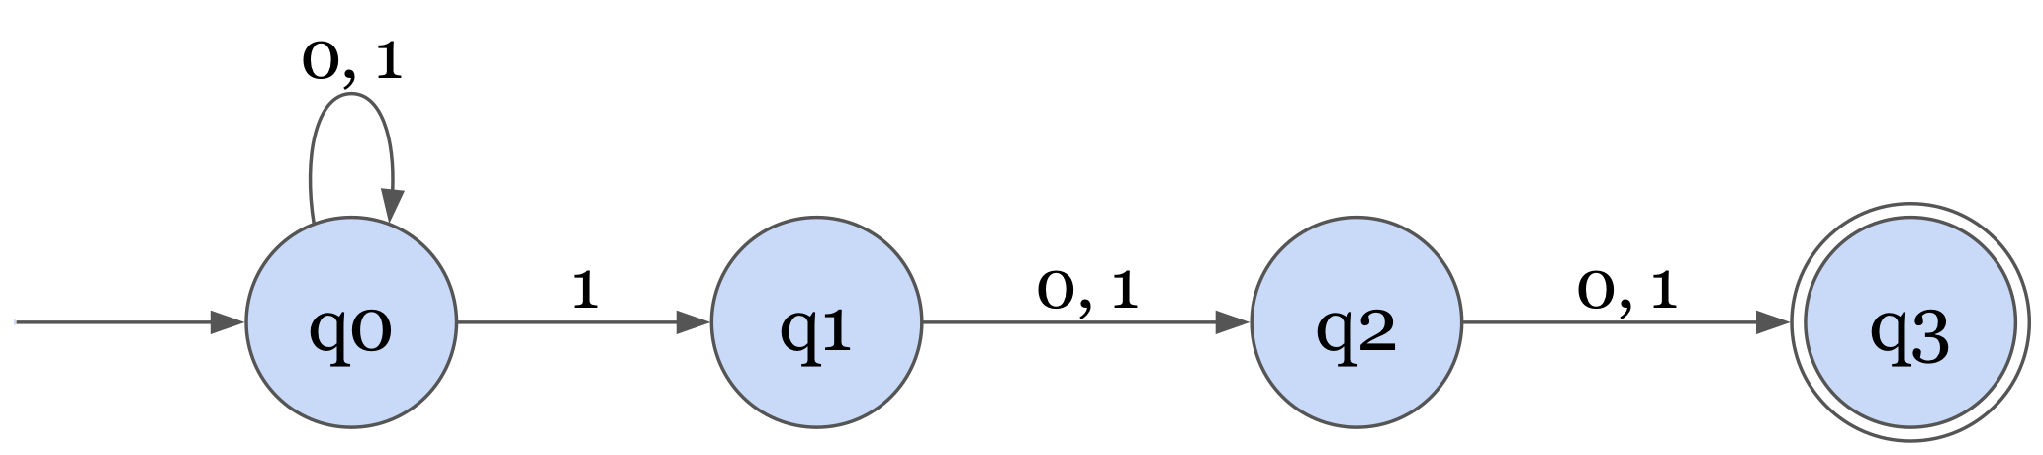
\includegraphics[width=\columnwidth]{figures/running_example_nfa}
  \caption{Running example: a 4-state NFA for binary strings whose third-to-last symbol is 1.}
  \label{fig:running}
\end{figure}

\section{Background and Related Work}
\label{sec:background}

Finite automata are mathematical models used to recognize regular languages. A deterministic finite automaton (DFA) has exactly one transition for each state and input symbol, while a nondeterministic finite automaton (NFA) can have multiple possible transitions, missing transitions, or transitions that consume no input ($\varepsilon$-transitions). Despite these differences, both DFAs and NFAs recognize the same class of languages, known as regular languages \cite{hopcroft2006introduction,sipser2006introduction}.

An NFA can be converted into an equivalent DFA using subset construction. For an NFA with $n$ states, the resulting DFA can have up to $2^n$ states. In this paper, we call families of NFAs that grow at an exponential rate when converted to DFAs ``blow-up'' NFAs. The blow-up family considered in this work recognizes $L_n$, the language of binary strings whose $n$-th symbol from the end is $1$. An NFA with $n+1$ states can recognize this language, while any equivalent DFA requires at least $2^n$ states. This lower bound can be proven using the pigeonhole principle \cite{malkin2018dfa}.

This theoretical result motivates our experiments. We first compare sparse, dense, and $\varepsilon$-transition NFA families to study how transition structures affect the number of reachable DFA states and the reduction achieved through minimization. The blow-up family serves as a worst-case comparison. After the limited findings of our initial experiment, we scale up and identify more specific NFA characteristics that influence the size and structure of equivalent DFAs.

\section{Methodology}
\label{sec:methodology}

\subsection{NFA Families}
\label{sec:families}

We begin with four random NFA families and the blow-up family, and later add a mixed family and its $\varepsilon$-variant, for six random families in all. The first four are \emph{sparse} (1--3 transitions drawn per state), \emph{dense} (4--7 transitions drawn per state), and their respective $\varepsilon$-variants, each augmented with 1--3 additional random $\varepsilon$-transitions. Transitions are drawn at random, so a repeated draw merges into one edge and a state can end up with fewer edges than drawn. The blow-up family consists of NFAs accepting the language in which the $n$-th symbol from the end of the input string must be $1$. Each automaton in this family has $n+1$ states, with $n$ ranging from 4 to 10. The \emph{mixed} family covers the generator settings that are neither sparse nor dense: its generator draws between a minimum and a maximum number of transitions per state, and the range straddles the sparse/dense boundary (for example 2--5 transitions per state), so a mixed NFA can have both sparsely and densely connected states. In the later experiments the class is determined from the range alone: sparse if the maximum is at most 3, dense if the minimum is at least 4, and mixed otherwise. In our experiments, we randomly generate NFAs, restricting them by the families described or by some other metric, convert them to DFAs using subset construction, minimize them with Moore's algorithm, and analyze the results.

\subsection{Subset Construction}
In the subset construction of an NFA, each state of the DFA represents a set of states in its parent NFA. This allows us to account for the nondeterminism of the NFA while operating within the DFA framework. When converting, the initial state is the $\varepsilon$-closure of $\{q_0\}$ in the NFA. For each DFA state, we use the NFA transition function to find all states reachable on each symbol of the alphabet. We then take the $\varepsilon$-closure of the resulting set to include all states reachable through $\varepsilon$-transitions. If the resulting set has not been encountered before, it is added to a BFS queue for further processing. A DFA state is accepting if it contains at least one NFA accepting state. The empty set serves as the dead state. \Cref{fig:subsettable} illustrates the construction for the running example, which results in 8 DFA states.

\begin{figure}[t]
  \centering
  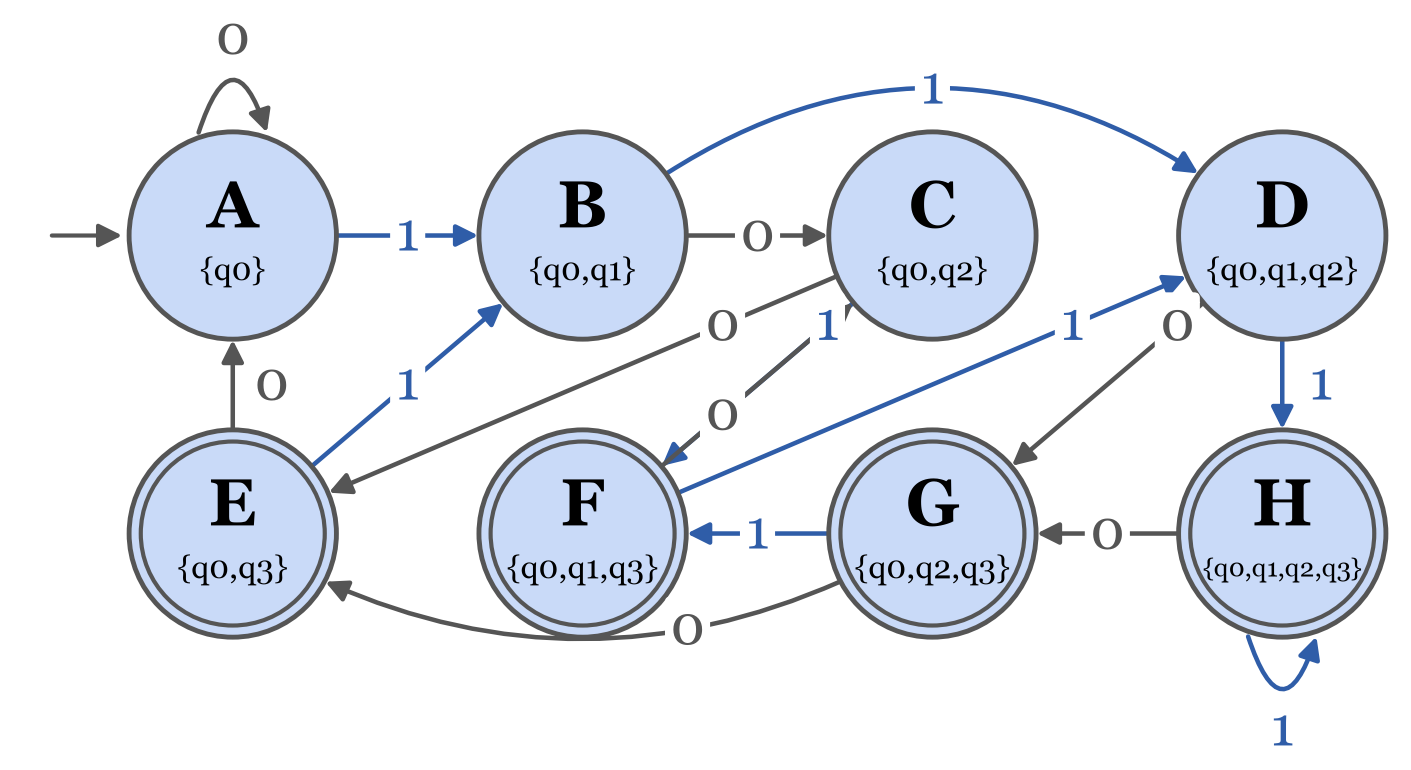
\includegraphics[width=\columnwidth]{figures/subset_table}
  \caption{Subset construction applied to the running example.}
  \label{fig:subsettable}
\end{figure}

\subsection{Moore Minimization}
Moore minimization starts by dividing the DFA states into two groups: accepting and non-accepting. Each group is repeatedly split whenever two states transition to different groups on the same input symbol. This process continues until no further splits are possible. In the running example, all eight states are distinguishable, so the DFA is already minimal.

\section{Implementation Details}
\label{sec:implementation}

We first implement an NFA generator that produces random NFAs with at least three states and a fixed alphabet, $\Sigma = \{0,1\}$. The generator allows us to specify the minimum and maximum number of transitions per state and whether $\varepsilon$-transitions are permitted. Each generated NFA has at least one and at most three accepting states.

To ensure that no unreachable states are included, we check the reachability of all states after generating each NFA. We treat the NFA as a graph and use depth-first search (DFS), starting from the initial state, to visit all reachable states. If any state remains unvisited, the NFA is rejected and a new one is generated. To avoid duplicate automata, we create a unique signature for each NFA using frozensets. The signature includes the states, alphabet, transitions, initial state, and accepting states. This allows us to identify and reject NFAs that have already been generated. In the million-NFA runs, we store a SHA-256 hash of this signature as the NFA's key. The ceiling search and the structured generator also treat an NFA and its copy with the symbols $0$ and $1$ swapped as the same NFA.

We convert each NFA into an equivalent DFA using the subset construction algorithm. Rather than generating all possible subsets of NFA states, we generate only those reachable from the initial DFA state. This avoids creating unnecessary states and makes the conversion more efficient.

\begin{algorithm}[t]
\caption{NFA-to-DFA Conversion Using Subset Construction}
\label{alg:subset}
\begin{algorithmic}[1]
\Require An NFA with states, alphabet, start state,
accepting states, and transitions,
and the helper functions $\textsc{EpsilonClosure}$ and $\textsc{Move}$
\Ensure An equivalent DFA

\State $start \gets \textsc{EpsilonClosure}(\{q_0\})$
\State $D \gets \{start\}$
\State $F_D \gets \emptyset$
\State $T_D \gets$ empty transition map
\State Initialize queue $Q$ with $start$

\While{$Q$ is not empty}
    \State $S \gets \textsc{Dequeue}(Q)$

    \If{$S \cap F \neq \emptyset$}
        \State $F_D \gets F_D \cup \{S\}$
    \EndIf

    \ForAll{$a \in \Sigma$}
        \State $M \gets \textsc{Move}(S,a)$
        \State $T \gets \textsc{EpsilonClosure}(M)$

        \If{$T \notin D$}
            \State $D \gets D \cup \{T\}$
            \State \textsc{Enqueue}($Q,T$)
        \EndIf

        \State $T_D[S,a] \gets T$
    \EndFor
\EndWhile

\State \Return $(D,\Sigma,start,F_D,T_D)$
\end{algorithmic}
\end{algorithm}

Subset construction does not guarantee a minimal DFA. Therefore, we apply Moore minimization to each converted DFA to obtain an equivalent minimized DFA.

\begin{algorithm}[t]
\caption{DFA Minimization Using Moore's Algorithm}
\label{alg:moore}
\begin{algorithmic}[1]
\Require A DFA with states, alphabet, start state, and accepting states
\Ensure An equivalent minimal DFA

\State $B \gets \textsc{InitialPartition}(DFA)$
\State $k \gets |\textsc{Unique}(B)|$

\Repeat
    \State $B \gets \textsc{RefinePartition}(DFA,B)$
    \State $k_{\text{new}} \gets |\textsc{Unique}(B)|$
\Until{$k_{\text{new}} = k$}
\State $S_{\min} \gets \textsc{Unique}(B)$
\State $q_{\min} \gets B[q_0]$
\State $F_{\min} \gets \{B[q] \mid q \in F\}$

\State Initialize $DFA_{\min}$ with
$(S_{\min},\Sigma,q_{\min},F_{\min})$

\ForAll{state $q$ of $DFA$}
    \ForAll{$a \in \Sigma$}
        \State $q' \gets \delta(q,a)$
        \State $\delta_{\min}(B[q],a) \gets B[q']$
    \EndFor
\EndFor

\State \Return $DFA_{\min}$
\end{algorithmic}
\end{algorithm}

To validate the construction and the minimization, we ran two independent checks that do not use the conversion code. The first is exact: it compares the NFA with its subset DFA, and the subset DFA with its minimized DFA, by exploring every pair of states that can be reached together and requiring that both members of every pair agree on acceptance. If they always agree, the automata accept the same language. We ran this check on every NFA in the first sweep, the 3,200-NFA sweep, the 10,000-NFA and million-NFA runs, the structured experiment, and the unrestricted comparison runs (about 12 million NFAs), and in the ceiling search on the ten NFAs it found; it never reported a disagreement. The second check is empirical: for each NFA we test 500 random input strings of length at most 20 and check that the NFA, the converted DFA, and the minimized DFA all accept or all reject each string. We ran it on every NFA in the first sweep (and in a 3,200-NFA sweep that preceded the 10,000-NFA run), the 10,000-NFA run, and the ten ceiling NFAs, and on a seeded 1\% sample (10,000 to 20,000 NFAs) of each million-NFA, structured, and unrestricted run; every string was classified consistently. These checks test the conversion and minimization, not whether the generator produces the NFAs we intend.

The project is implemented in Python 3, using DuckDB and JSON for data storage, and Matplotlib, Seaborn, and Graphviz for visualization. The initial implementation is provided in a self-contained Jupyter notebook. For subsequent experiments, the code base was modularized, and each experiment is roughly contained in one file that uses the modules. A seeded random number generator (RNG) is used to ensure reproducibility of results, and symbols are drawn from a sorted alphabet so that a seed gives the same NFA in every run. For analyzing large numbers of randomly generated NFAs, DuckDB stores each NFA's identity, class, structural features, and the number of DFA states after subset construction and after minimization. The NFAs of the smaller runs are saved as JSON files; for the million-NFA runs, we keep each NFA's seed and key instead, from which the NFA can be regenerated. Additionally, a visualization module generates graphical representations of arbitrary NFAs and DFAs.

\section{Experiments, Results, and Analysis}
\label{sec:results}

\subsection{Setup and Measures}
\label{sec:setup}

Each experiment draws random NFAs from the generator, converts them with subset construction, minimizes the result, and compares the sizes of the NFA and its two DFAs (\cref{tab:runs}). The generator settings for each run are given with its results. NFAs are grouped into the sparse, dense, and mixed classes, and their $\varepsilon$ variants, by the transition range with which they were generated. Our main measurement is the size ratio: the number of DFA states divided by the state count of the parent NFA. We compare against the NFA as generated and do not minimize it first, so redundant NFA states make the DFA look smaller than it would against a minimal NFA. When searching for the largest possible DFAs, we use the ceiling of $2^n$ states, the largest size a minimized DFA can reach relative to its parent NFA \cite{sipser2006introduction}. In the trait analysis, an NFA is considered \emph{extreme} if its minimized DFA is in the top 5\% for its class and state count.

\begin{table}[t]
  \centering
  \caption{The experiments.}
  \label{tab:runs}
  \small
  \begin{tabular}{@{}lp{2.0cm}lp{2.3cm}@{}}
    \toprule
    Run & NFAs & States & Purpose \\
    \midrule
    First sweep & 50 per class, 4 classes; blow-up family & 10; 5--11 & Compare classes \\
    Balanced & 10,000 & 5--12 & Compare classes; find traits \\
    Trait tests & 12,000 fresh; $10\times4{,}000$ paired & 5--12 & Replicate; change one trait \\
    Large random & 1M $\times$ 3 runs; 2.5M new & 5--12, 6, 12 & Approach to ceiling; hunt for hits \\
    Structured & 1M structured vs.\ 1M random, per size & 5, 6, 7 & Generate only the hit shape \\
    \bottomrule
  \end{tabular}
\end{table}

\subsection{Initial Experiment}
\label{sec:first}

We started with 50 random NFAs of 10 states in each of four classes (sparse, dense, sparse-$\varepsilon$, dense-$\varepsilon$), plus the blow-up family. \Cref{tab:small} gives the averages. Subset construction made the machine larger for most NFAs, between 70\% (dense-$\varepsilon$) and 100\% (sparse) of them. After minimization, dense NFAs lost about 73\% of their states (20.2 to 5.5 on average), while sparse NFAs lost only 17\% (35.8 to 29.9), and 98\% of sparse NFAs had a larger DFA. At this scale, the sparse classes are the ones where the DFA stays large. One clear oversight of this first experiment and those that follow is the handling of $\varepsilon$ edges. Our analysis of the effect of $\varepsilon$ edges could have been more robust had we also replaced edges with $\varepsilon$ transitions instead of randomly adding them on top of the existing NFAs.

\begin{table}[t]
  \centering
  \caption{Average DFA size for 50 NFAs of 10 states per class.}
  \label{tab:small}
  \small
  \begin{tabular}{@{}lrrrr@{}}
    \toprule
    Class & Subset & Minimized & \% larger (subset) & \% larger (min.) \\
    \midrule
    Sparse & 35.8 & 29.9 & 100 & 98 \\
    Sparse-$\varepsilon$ & 25.5 & 18.2 & 94 & 70 \\
    Dense & 20.2 & 5.5 & 92 & 14 \\
    Dense-$\varepsilon$ & 12.8 & 4.0 & 70 & 2 \\
    \bottomrule
  \end{tabular}
\end{table}

The blow-up family behaves significantly differently from the rest (\cref{fig:blowup}). For $n=4,\dots,10$, the DFA has exactly $2^n$ states, and minimization has no effect on the size. To illustrate the extremity of this effect, the largest minimized DFA among the 200 random NFAs had 70 states, while the blow-up NFA with 10 states produces 512 states in the minimized DFA. From this experiment, we gathered that NFA sparsity is an influential factor in determining the space complexity of a minimized DFA, as the sparse NFAs were far harder to minimize and adding $\varepsilon$ edges decreased the average size of the DFA in both cases. This is intuitive, as denser NFAs will likely have a greater amount of redundancy and therefore stand a greater chance of benefiting from DFA minimization. The blow-up class behaved exactly as expected.

\begin{figure}[t]
  \centering
  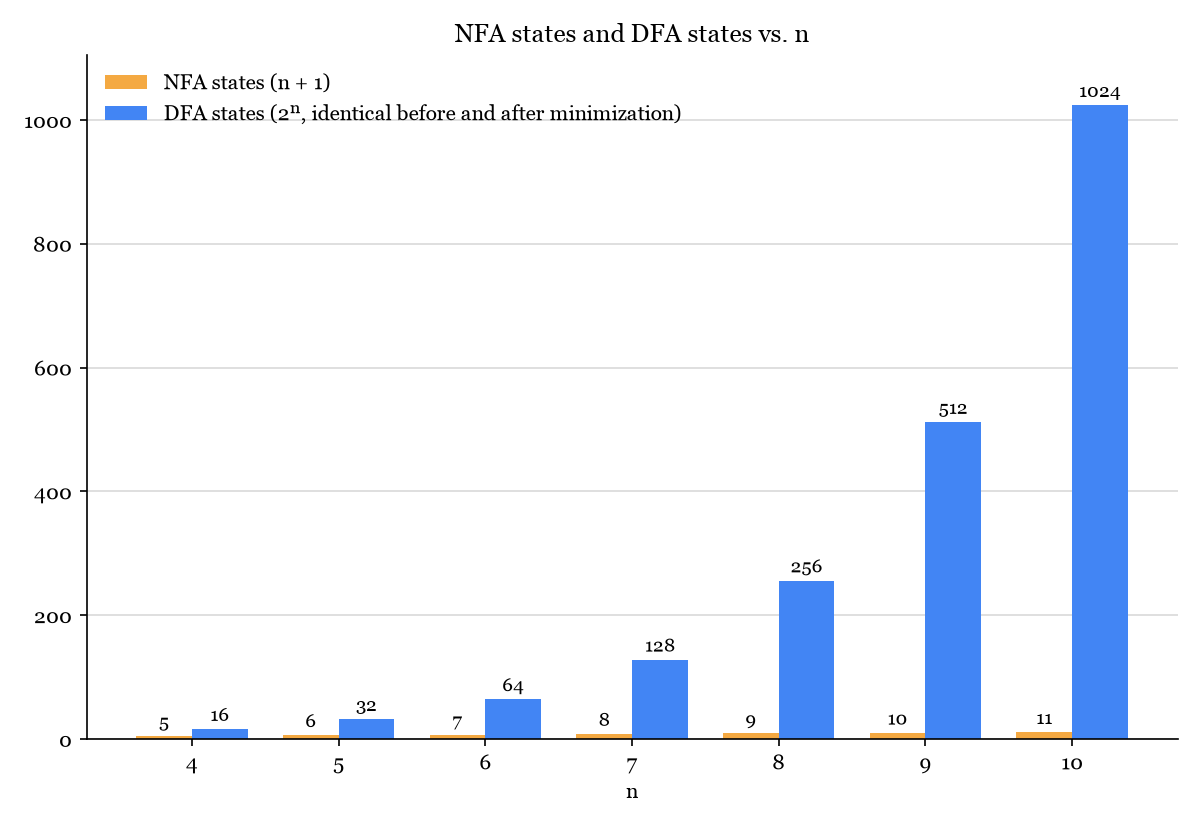
\includegraphics[width=\columnwidth]{figures/blowup_family}
  \caption{NFA states ($n{+}1$) and DFA states ($2^n$) for the blow-up family.}
  \label{fig:blowup}
\end{figure}

\subsection{Scaling Up the Initial Experiment}
\label{sec:10k}

To check that our observation about sparsity held with more data, we generated 10,000 random NFAs with 5 to 12 states, split evenly over the six classes.

\Cref{fig:vs} compares each NFA with its two DFAs. The subset DFA is larger a majority of the time for all of the classes, which is expected. After minimization, the share of larger DFAs drops to about what we would expect given our initial experiment (\cref{fig:vs}, bottom). Minimization removes most of the growth for dense NFAs and very little of it for sparse ones. Among the NFAs that do end up larger, the typical growth is modest (\cref{fig:tenk}, left): the median ratio goes from 2.3$\times$ for sparse down to 1.3$\times$ for dense-$\varepsilon$. However, many outlying DFAs are far larger than their parent NFAs. The largest ratio in this run was 28$\times$, an NFA with 9 states and a minimized DFA of 255 states.

\begin{figure*}[!t]
  \centering
  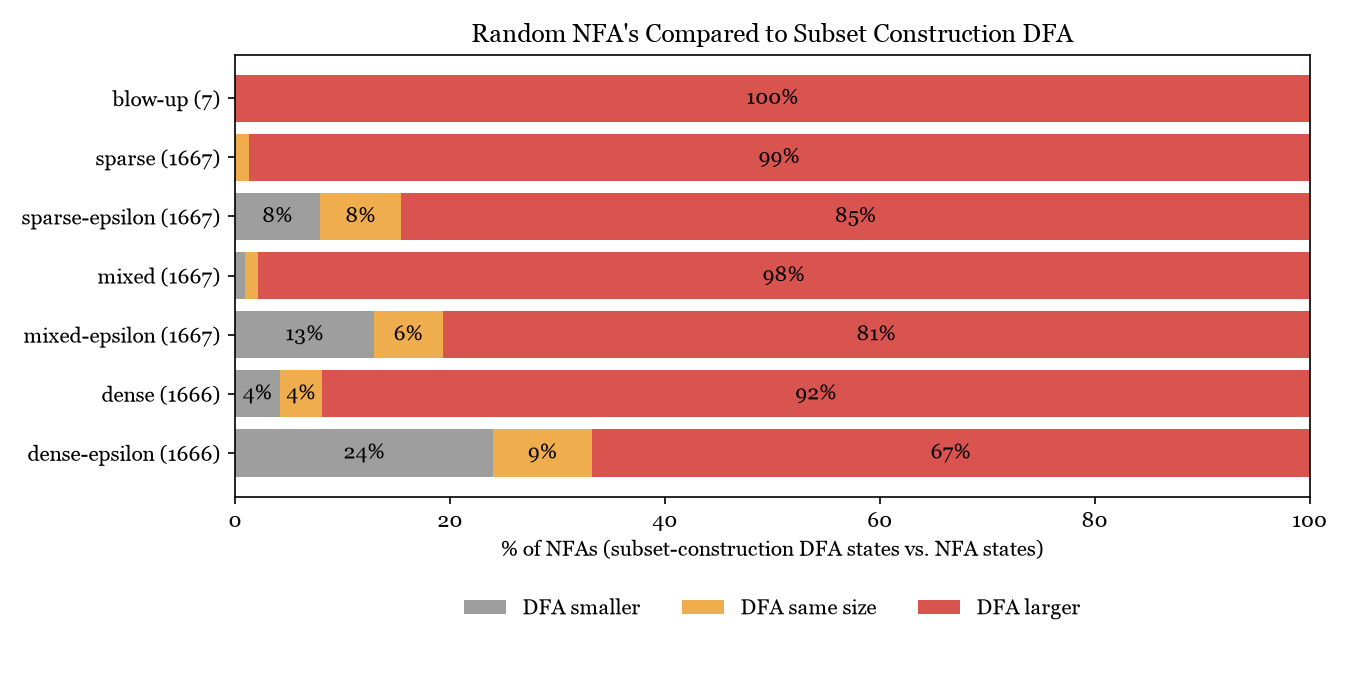
\includegraphics[width=0.8\textwidth]{figures/vs_subset}\\[4pt]
  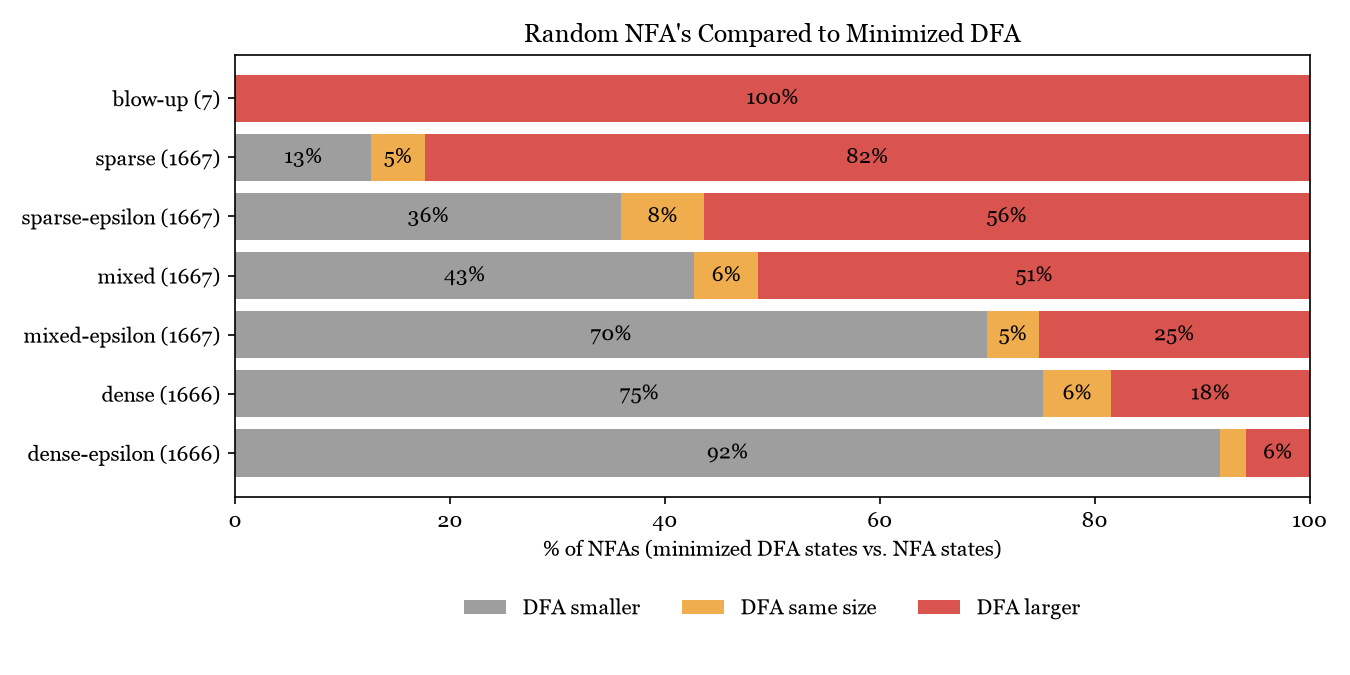
\includegraphics[width=0.8\textwidth]{figures/vs_minimized}
  \caption{Random NFAs compared to (top) their subset-construction DFA and (bottom) their minimized DFA.}
  \label{fig:vs}
\end{figure*}

The more important observation is how close the DFA sizes get to their ceiling (\cref{fig:tenk}, right). The best NFA in the run reaches 69\% of its $2^n$ ceiling, and only 41 of the 10,000 have a minimized DFA larger than $2^{3n/4}$. For dense NFAs, most of the growth that subset construction produces is redundant and is removed by minimization (the mean size ratio falls from 2.2 to 0.75), but for sparse NFAs little of it is (3.1 to 2.4), and what remains rarely approaches the ceiling.

An NFA with $\varepsilon$ edges is less likely to grow than a plain NFA of the same density. This does not mean that $\varepsilon$ edges are good for compactness in general. In our generator, they are added on top of the ordinary transitions, so an NFA with them has more edges than its non-$\varepsilon$ counterpart, and $\varepsilon$-closures probably cause many subsets to coincide. We return to this when testing changes below.

\begin{figure*}[!t]
  \centering
  \begin{minipage}[t]{0.48\textwidth}
    \centering
    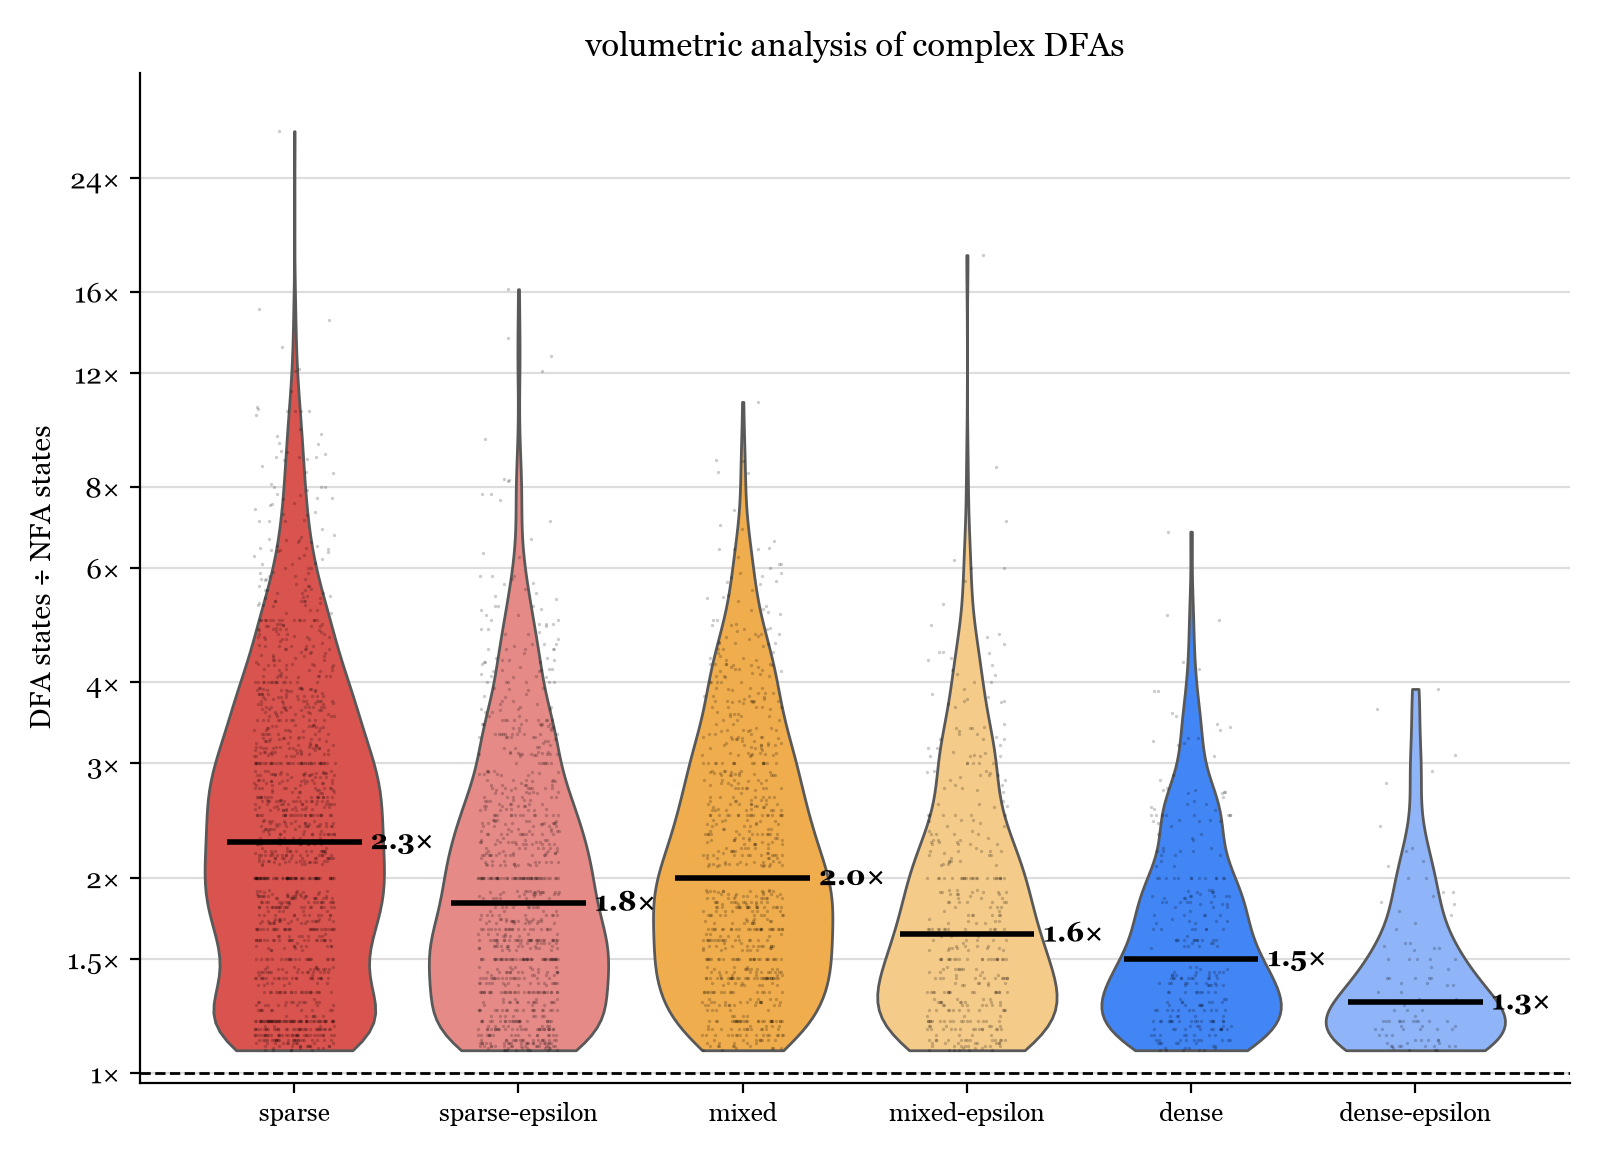
\includegraphics[width=\linewidth]{figures/violin}
  \end{minipage}\hfill
  \begin{minipage}[t]{0.48\textwidth}
    \centering
    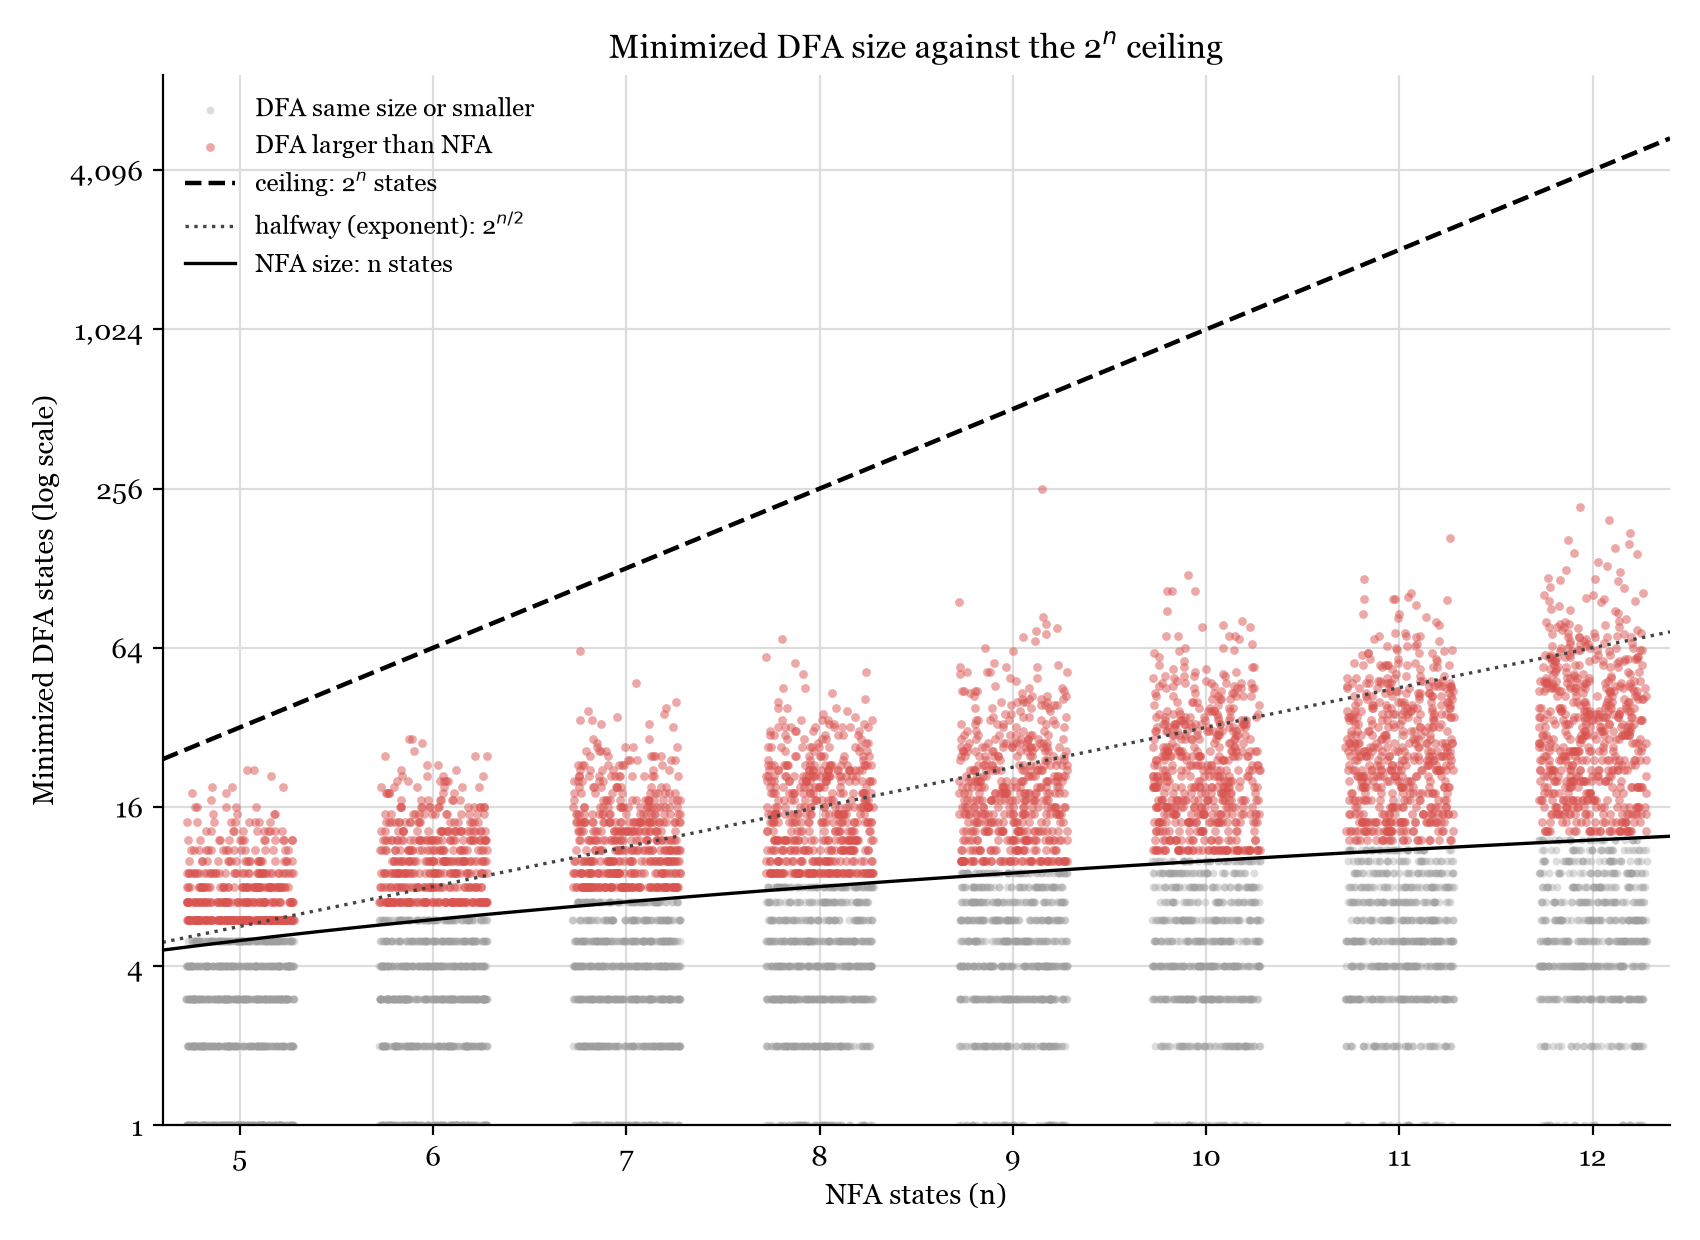
\includegraphics[width=\linewidth]{figures/ceiling_scatter}
  \end{minipage}
  \caption{The 10,000-NFA run. (Left) DFA/NFA state ratio, only for DFAs larger than their NFA. (Right) Minimized DFA size against the $2^n$ ceiling.}
  \label{fig:tenk}
\end{figure*}

\subsection{Analyzing NFA Outliers}
\label{sec:traits}

To see what separates the large DFAs from the rest, we took the 520 extreme NFAs from the 10,000 (the top 5\% grouped by class type and state number) and compared them on 24 structural traits. First, each trait was standardized within its group. Nineteen of the 24 differ from the rest at a Bonferroni-corrected level of $p<0.002$. Generally, the extreme NFAs have less branching (1.65 destinations per defined (state, symbol) pair against 1.86), lower out-degree (3.0 against 3.4), fewer accepting states (1.7 against 2.0), and fewer $\varepsilon$ edges (0.76 against 1.03).

Looking at how the share of extreme NFAs changes with each trait (\cref{tab:traits}) is more informative, because the relationship is often not monotonic. One clear case is nondeterminism. NFAs with 0.25 to 0.75 nondeterministic (state, symbol) pairs per state are extreme about 8\% of the time, compared with 5.2\% overall, but NFAs with very little of it (3.8\%) and with a lot of it (1.3\% above 1.5 per state) are less likely to be extreme. This correlates with our previous sparsity observation. Too little nondeterminism leaves the subset construction nothing to track, and too much makes the reachable subsets collapse into the same few sets, which minimization then merges. The other traits are easier to state: one accepting state, that state three or so steps from $q_0$, few $\varepsilon$ edges, and a single strongly connected component. A random forest on these traits predicts extremeness with a cross-validated AUC of 0.82. The traits carry real information about which NFAs are extreme but do not determine it.

\begin{table}[t]
  \centering
  \caption{Share of NFAs whose minimized DFA is extreme, by trait value (baseline 5.2\%). Highest rate in each row in bold.}
  \label{tab:traits}
  \small
  \begin{tabular}{@{}ll@{}}
    \toprule
    Trait & Values $\rightarrow$ \% extreme \\
    \midrule
    Non-det.\ pairs per state & $\le$0.25: 3.8 \;\; 0.25--0.5: \textbf{8.4} \;\; 0.5--0.75: 7.9 \;\; 0.75--1.0: 6.6 \;\; 1.0--1.5: 4.9 \;\; $>$1.5: 1.3 \\
    Accepting states & 1: \textbf{8.0} \;\; 2: 4.4 \;\; 3: 3.2 \\
    Distance to accepting state & 0: 4.5 \;\; 1: 4.3 \;\; 2: 6.5 \;\; 3: \textbf{9.0} \;\; 4: 7.3 \;\; 5+: 3.5 \\
    $\varepsilon$ edges ($\varepsilon$ classes) & 1: \textbf{10.0} \;\; 2: 4.7 \;\; 3: 1.5 \\
    Single strongly connected component & yes: \textbf{5.7} \;\; no: 2.1 \\
    \bottomrule
  \end{tabular}
\end{table}

We verified these traits in two ways. First, we generated 12,000 new NFAs and called an NFA a \emph{profile} match if it had one accepting state, an accepting state at distance 2 or more, and 0.25 to 1.0 nondeterministic pairs per state. Using the extreme thresholds from the first 10,000, 9.11\% of the 955 matching NFAs were extreme, against 4.73\% of the others. The profile helped for mixed and dense NFAs but not for sparse ones, whose generator already tends to produce this shape.

Second, we changed one trait at a time on the same NFAs and rebuilt the DFA, so every comparison is paired (\cref{fig:traits}). Each test used up to 4,000 NFAs (fewer when a change did not apply to every NFA) and was repeated on ten independent samples. Moving toward the profile made the DFA grow in 54--66\% of NFAs and shrink in 10--17\%. In two control experiments (adding accepting states and adding an edge to every state), the DFA shrank for 48\% and 52\% of NFAs and grew for 9\% and 17\%. The intervals across the ten replications are about a point wide, so the direction does not seem to be an accident of one sample. However, the measured increase is modest. The median change is 1.1 to 1.4 times, and the means are higher only because of a few outlying NFAs. Deleting $\varepsilon$ edges grew the DFA for 57\% of NFAs, but this test is confounded, since an NFA without them moves into a class where DFAs tend to be larger, which is why we rely more on the within-class comparison above. To reach a substantial size difference, more than one of the discovered traits is needed at once.

\begin{figure*}[!t]
  \centering
  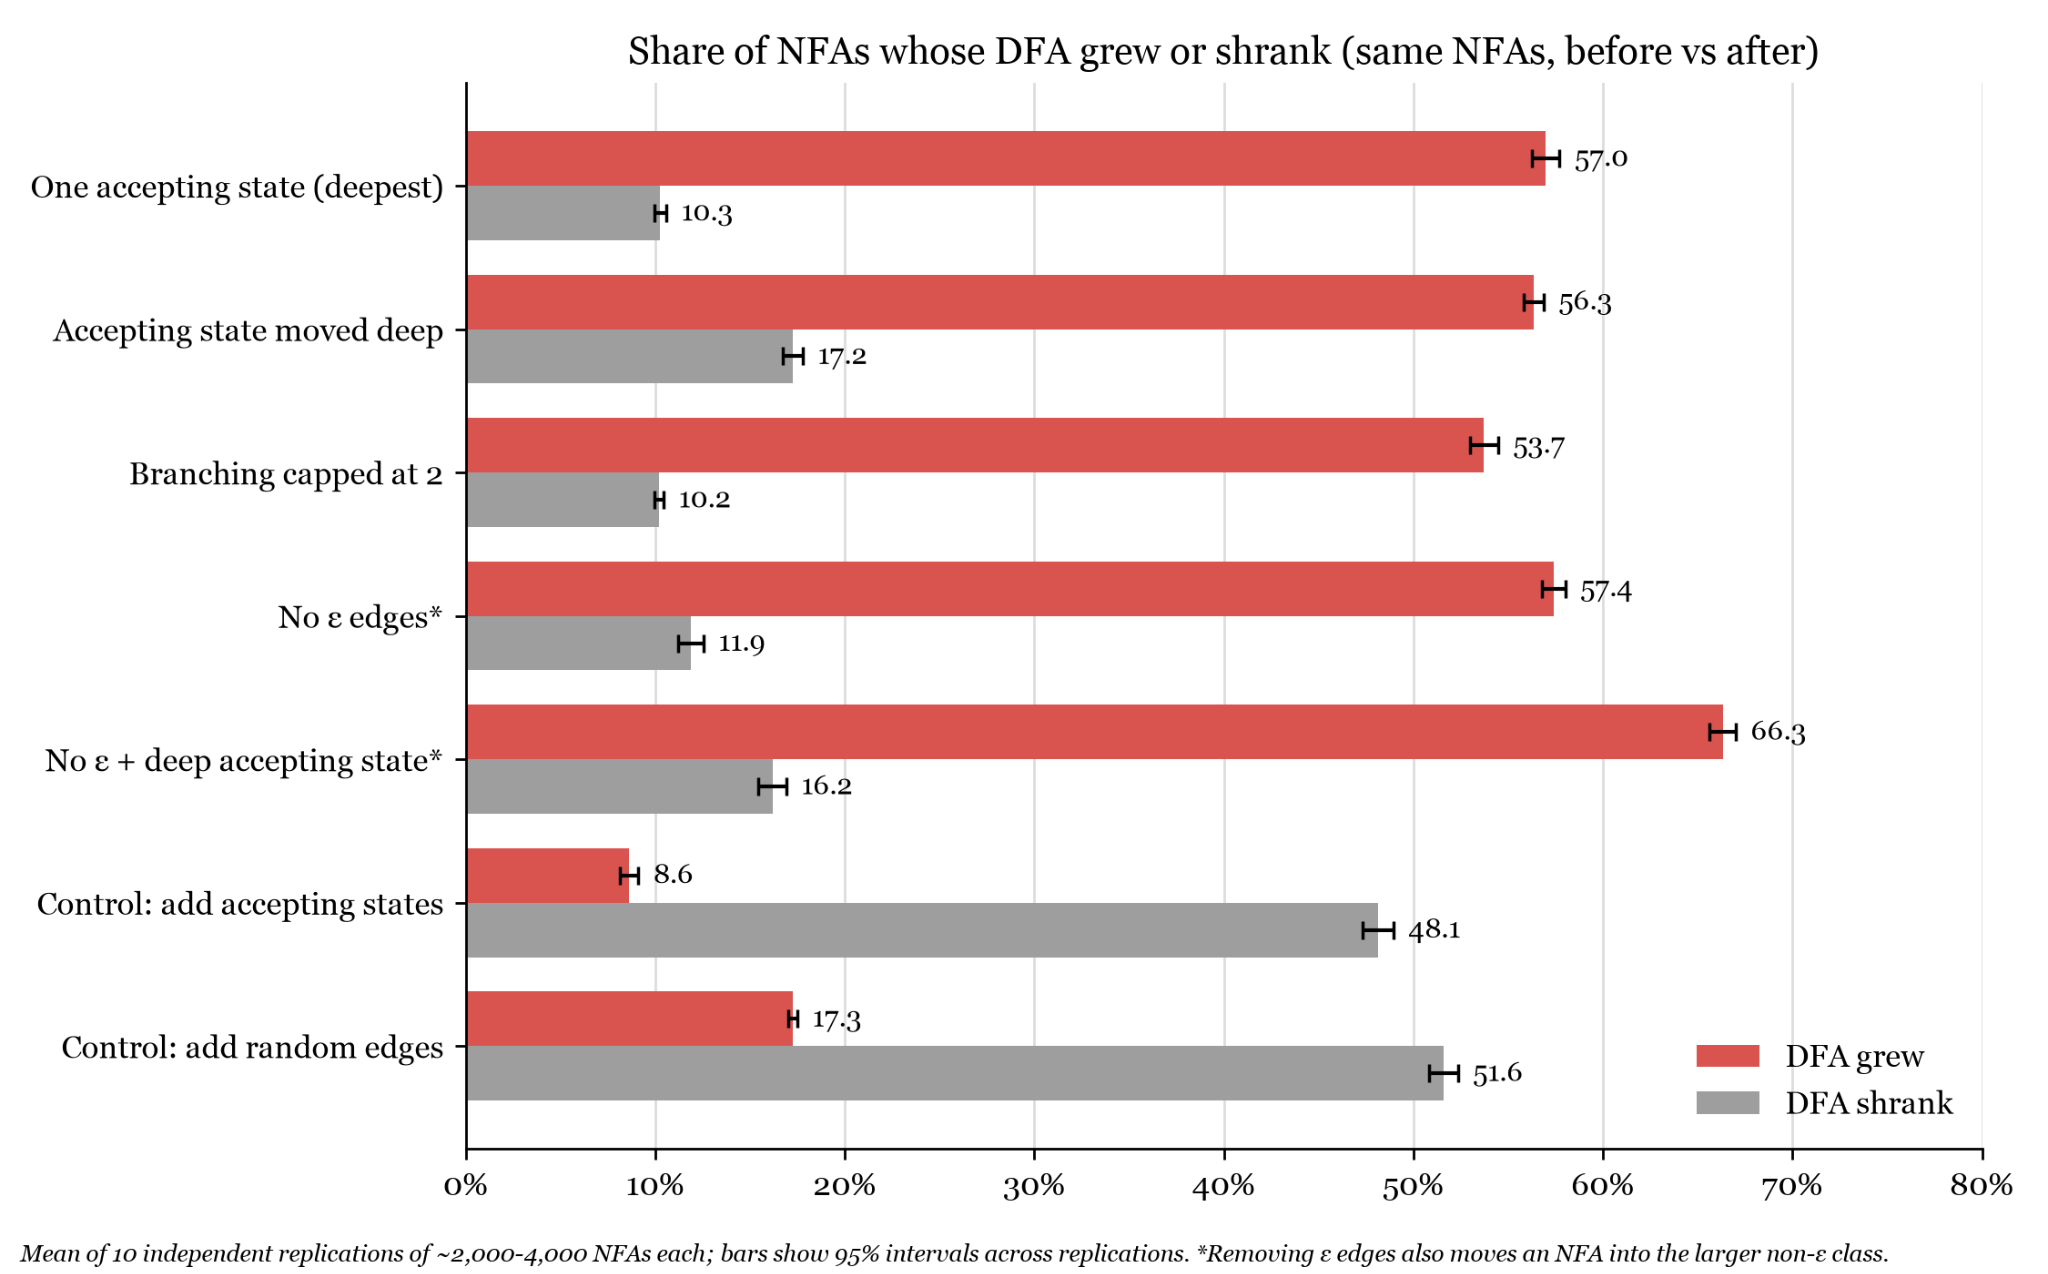
\includegraphics[width=0.8\textwidth]{figures/trait_tests}
  \caption{Share of NFAs whose DFA grew or shrank after each one-at-a-time change. Bars show 95\% intervals across ten replications. The remaining 18--43\% of NFAs kept the same number of states. *Removing $\varepsilon$ edges also moves an NFA into the larger non-$\varepsilon$ class.}
  \label{fig:traits}
\end{figure*}

\subsection{Searching for Worst-Case NFAs}
\label{sec:ceiling}

To get a better sense of how close random NFAs can get to the $2^n$ ceiling, we rescaled the experiment. In a run of one million NFAs with 5 to 12 states, three reached their ceiling. However, the NFAs that do are small. When this experiment was repeated with only six-state NFAs, one NFA reached the 64-state ceiling (\cref{fig:hexbin}).

\begin{figure*}[!t]
  \centering
  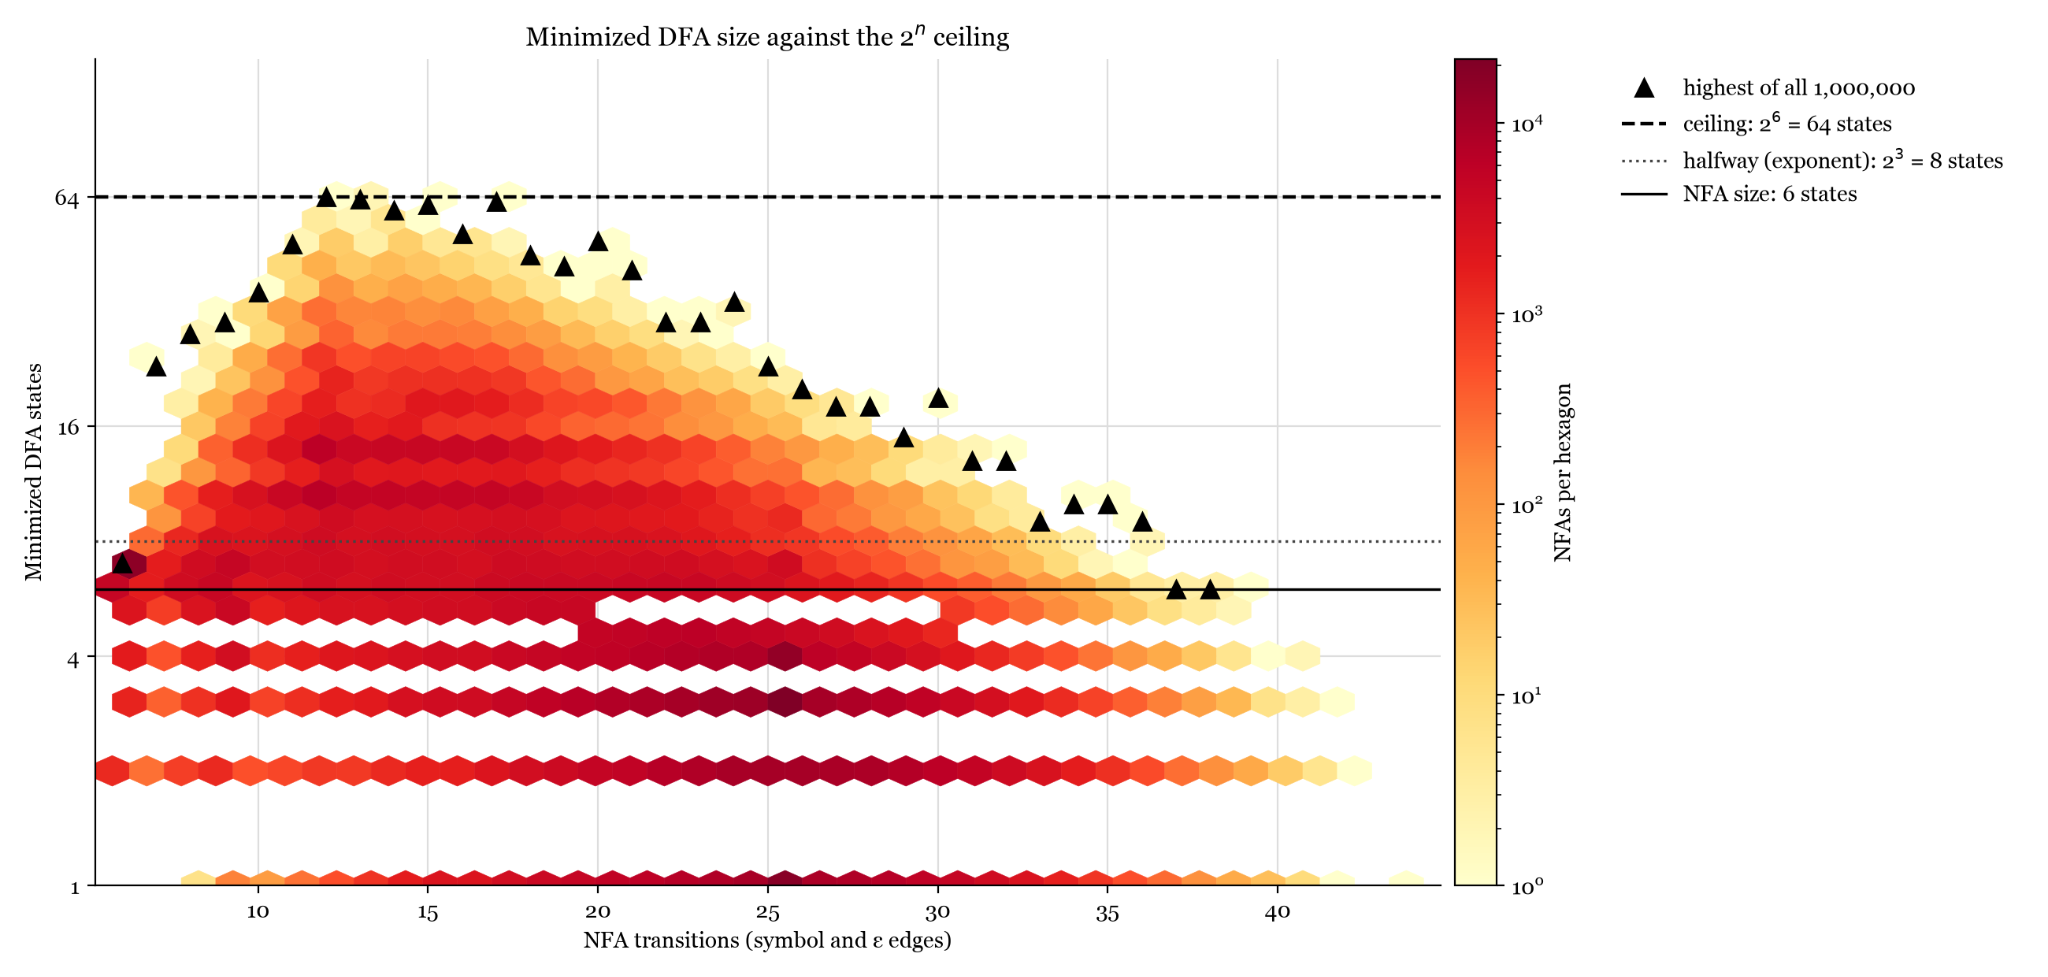
\includegraphics[width=0.8\textwidth]{figures/hexbin_6_states}
  \caption{Minimized DFA size of 1M random 6-state NFAs against the ceiling. Colour shows the number of NFAs in each hexagon (log scale), and triangles mark the largest DFA found at each transition count.}
  \label{fig:hexbin}
\end{figure*}

We changed the search to continue drawing distinct 6-state NFAs until ten worst-case NFAs were discovered. Scanning 2,517,323 new NFAs took 68 seconds and gave nine new hits, about 3.6 per million. Together with the one from the previous million-NFA run, these are the ten NFAs we examined. All ten are sparse and have no $\varepsilon$ edges, one to three nondeterministic pairs, one to three accepting states, and exactly one state that does not account for every symbol in the alphabet. Every DFA contains all 64 subsets, including the empty set, and minimization merges none. Interestingly, these NFAs are very close to deterministic. \Cref{fig:ceilingnfa} shows one of them.

\begin{figure}[t]
  \centering
  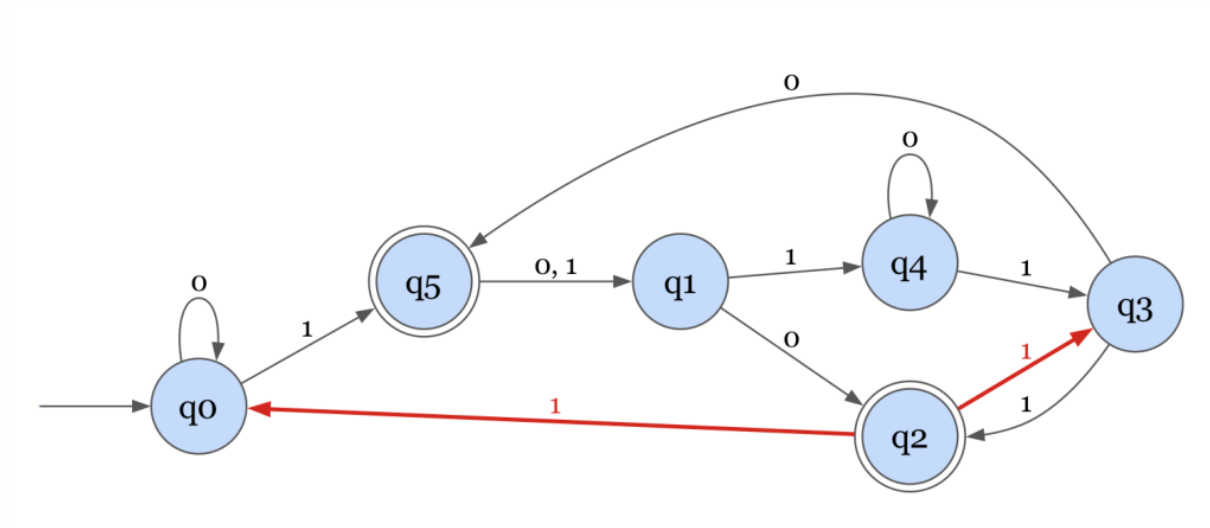
\includegraphics[width=\columnwidth]{figures/ceiling_nfa}
  \caption{A 6-state NFA whose minimized DFA reaches the 64-state ceiling.}
  \label{fig:ceilingnfa}
\end{figure}

\subsection{Structured NFA Generation}
\label{sec:structured}

To test whether these observed traits truly drive DFA complexity, we implemented a generator that randomly produces NFAs with these traits. The structured generator builds an $n$-state NFA with no $\varepsilon$ edges and one to three accepting states, leaves one of the $2n$ (state, symbol) slots empty (chosen uniformly), gives every other slot one random destination, and then adds a second destination to one to three of the defined slots. NFAs that fail the reachability check are redrawn. For 5, 6, and 7 states, we generated one million distinct structured NFAs and compared them with one million unrestricted NFAs of the same size, also without $\varepsilon$ edges.

The shape raises the median DFA size by a factor of about two to three at every size and drastically increases the odds of discovering complex DFAs (\cref{tab:structured_vs_unrestricted_nfas}). The gap widens as $n$ grows. At 6 states, 116 structured NFAs per million reach the ceiling against 3 in the random run. At 7 states, the ratio is 30 to 0. Reaching the ceiling still gets rarer with size (608, 116, and 30 per million), so the shape improves the odds without removing the difficulty of large $n$. Because we have few ceiling hits in our random run, the ceiling ratios are not very precise. The half-ceiling column rests on many more NFAs per row and is a more reliable comparison.

\begin{table*}[t]
\centering
\caption{Structured vs. Unrestricted NFAs}
\label{tab:structured_vs_unrestricted_nfas}
\begin{tabular}{@{}llrrrrr@{}}
\toprule
\textbf{NFA States} & \textbf{Generator} & \textbf{Median DFA} & \textbf{DFA $\ge \frac{1}{4}$} & \textbf{DFA $\ge \frac{1}{2}$} & \textbf{DFA $\ge \frac{3}{4}$} & \textbf{DFA at} \\
 & &  \textbf{States} & \textbf{of Ceiling} & \textbf{of Ceiling} & \textbf{of Ceiling} & \textbf{Ceiling} \\
\midrule
\multirow{3}{*}{5 states}
 & structured & 9 & 61.4\% & 11.4\% & 1.17\% & 608 \\
 & unrestricted & 5 & 24.9\% & 1.72\% & 0.0816\% & 34 \\
 & \textbf{ratio} & \textbf{1.8$\times$} & \textbf{2$\times$} & \textbf{7$\times$} & \textbf{14$\times$} & \textbf{18$\times$} \\
\addlinespace
\multirow{3}{*}{6 states}
 & structured & 13 & 38.6\% & 3.77\% & 0.287\% & 116 \\
 & unrestricted & 6 & 7.48\% & 0.215\% & 0.0087\% & 3 \\
 & \textbf{ratio} & \textbf{2.2$\times$} & \textbf{5$\times$} & \textbf{18$\times$} & \textbf{33$\times$} & \textbf{39$\times$} \\
\addlinespace
\multirow{3}{*}{7 states}
 & structured & 20 & 19\% & 1.14\% & 0.0929\% & 30 \\
 & unrestricted & 7 & 1.43\% & 0.0255\% & 0.0006\% & 0 \\
 & \textbf{ratio} & \textbf{2.9$\times$} & \textbf{13$\times$} & \textbf{45$\times$} & \textbf{155$\times$} & \textbf{30 vs 0} \\
\bottomrule
\end{tabular}
\end{table*}

\subsection{Discussion}
\label{sec:discussion}

We set out to measure DFA size across NFA families, to find out when minimization helps, and to identify what makes some NFAs blow up. The first two are answered directly in our experiments. Subset construction makes the machine larger for most random NFAs (87\% of the 10,000), minimization removes most of that growth for dense NFAs and little for sparse ones, and for the blow-up family it removes nothing. The third is answered in part. We can describe the NFAs that blow up (nearly deterministic, a small amount of nondeterminism, few accepting states placed some distance from the start, few $\varepsilon$ edges), we checked this on fresh NFAs and by changing one trait at a time, and a generator built around the shape reaches at least half the ceiling 7 to 45 times more often than a random one. What we cannot say is which part of the shape does the work, because the structured generator fixes its three ingredients together, or why these NFAs are hard, since we have not looked at the languages they accept.

Two results surprised us. The first is that more nondeterminism does not give a larger DFA. Dense NFAs have more nondeterminism, yet their minimized DFAs are mostly smaller than the NFA (75\% of dense NFAs in the 10,000 run). We suspect that in dense NFAs the subsets collapse into a few repeated sets, but we did not check the languages directly. The second is how rarely random NFAs get near the ceiling. At 6 states, the ceiling is a rare event under random generation, about 3.6 in a million in our search. The blow-up family shows that exponential growth can be reached with a very simple NFA, but random generation rarely finds this sort of structure.

The results have several limits. Almost all NFAs have between 5 and 12 states over a two-letter alphabet, and the searches for the ceiling cover only 5 to 7 states (plus one random run at 12), so we do not know that the traits carry over to larger NFAs or other alphabets. Our statements about random NFAs describe one generator, in which transitions are drawn with replacement and the density classes are defined by the number of draws; another generator could give different shares. We compare against the NFA as generated and never minimize it, so some NFAs contain redundant or useless states that make the DFA look smaller by comparison. The traits were found on one data set and checked on fresh NFAs from the same generator, so the checks do not show that they hold for NFAs produced any other way, and our random NFAs may not resemble the automata that arise from real regular expressions or languages. The one-at-a-time changes alter the language an NFA accepts, so they show that structure drives size, not that a particular language has a smaller or larger DFA, and the confidence intervals in those tests cover which NFAs were drawn and which edges each change picked, but not the choice of generator, extreme threshold, or alphabet. The structured generator fixes its three ingredients together, so it cannot attribute the gain to any one of them, and its shape was read off only ten six-state NFAs. Our handling of $\varepsilon$ edges is also weak, since we added them on top of existing transitions instead of replacing transitions, so the effect of $\varepsilon$ edges is mixed in with the effect of having more edges. Finally, the random-string equivalence check ran on a 1\% sample of the million-NFA runs, not on every NFA, and in the ceiling search only the ten hits were checked, not every NFA scanned. 

\section{Conclusion and Future Work}
\label{sec:conclusion}

We measured how large a DFA becomes when nondeterminism is removed from random NFAs and what drives that growth. Subset construction makes the machine larger for most random NFAs, but minimization removes most of that growth for dense NFAs: in the 10,000-NFA run, 18\% of dense NFAs ended with a larger minimized DFA, against 82\% of sparse ones. The blow-up family is the opposite, growing exponentially with nothing for minimization to remove. Reaching the $2^n$ ceiling by chance is rare, about 3.6 in a million at 6 states, and the NFAs that do reach it share a recognizable shape: sparse, nearly deterministic, with one missing transition, a few nondeterministic choices, and few accepting states, all with no $\varepsilon$ edges. Generating only that shape reaches at least half the ceiling 7 to 45 times more often at 5 to 7 states. For the question we started with, this suggests that determinizing is expensive for a narrow class of NFAs, those that are close to deterministic but carry a small amount of well-placed nondeterminism, and cheap for most others, including dense ones, which usually shrink.

Several questions remain open. Our random generation could be replaced by generation from languages or regular expressions to test whether these traits appear in practical automata. The one-at-a-time and structured experiments could be extended to separate the ingredients of the structured shape and to replace transitions with $\varepsilon$ edges instead of adding them. Larger NFAs and alphabets would show whether the traits scale, and the patterns of state growth in the worst-case NFAs, as in the blow-up family, could be analyzed formally to explain why these structures are hard. Finally, the exact equivalence check could be extended to every NFA scanned in the ceiling search, not only the hits, and the random-string check to every NFA in the million-NFA runs.

\section{Declaration of Generative AI Use}
\label{sec:genai}

Claude and ChatGPT were used to assist with report drafting and editing, while Claude, Claude Code, ChatGPT, and Microsoft Copilot were used as coding assistants for development and debugging. All AI-generated content and code were reviewed and modified by the authors, who take responsibility for the final work.

\section*{Member Contributions}
\label{sec:contributions}

\begin{itemize}
    \item \textbf{Cole Kelley:} Designed and ran the experiments; co-wrote the presentation and report.
    \item \textbf{Sifat Moonjerin:} Developed the initial framework; co-wrote the presentation and report.
\end{itemize}

\bibliographystyle{IEEEtran}
\bibliography{refs}

\end{document}
